\documentclass{article}
\usepackage[spanish]{babel}
	\deactivatetilden
\spanishdecimal{.}
\addto\captionsspanish{\def\tablename{Tabla}}
\addto\captionsspanish{\def\listtablename{\'Indice de tablas}}
\usepackage[numbers,sort&compress]{natbib}
\usepackage[T1]{fontenc}
\usepackage[utf8]{inputenc}
\usepackage{graphicx}
\usepackage{url}
\usepackage{graphicx}
\graphicspath{{Figuras/}}
\usepackage[numbers,sort&compress]{natbib}
\usepackage[clearempty,pagestyles]{titlesec}
\usepackage{anysize}
\usepackage{xcolor, colortbl}
\usepackage{array, multirow, multicol}
\usepackage{enumerate} 

\def\baselinestretch{1.5}
\papersize{27.9cm}{21.5cm} 
\marginsize{2cm}{2cm}{1cm}{1cm}

\title {Sistema Multiagente}
\author{Julio Garc\'ia}
\pagestyle{empty}

\pagestyle{empty}
\begin{document}
	\renewcommand{\listtablename}{Índice de tablas}
	\renewcommand{\tablename}{Cuadro}
	\maketitle
	
	\section{Introducción}
	En el presente trabajo se busca como objetivo principal la modificación del modelo SIR (Susceptibles, Infectados, Recuperados). Esta versión del sistema modelo SIR, utilizado en epidemiología, se basa en la variante de que uno de los agentes puede ser vacunado en su creación y esto le daría inmunidad a la infección modelada.\\
	En la tarea de la práctica 6 \cite{p6} se busca estudiar el efecto que tiene el porcentaje de vacunación en el porcentaje de contagiados activos en un momento dado y en el tiempo en el que se alcanza el porcentaje máximo de contagios activos.
	
	\section{Desarrollo}
	En este trabajo se estudia la cantidad de iteraciones necesarias (momento del tiempo) en el que es alcanzado el porcentaje máximo de contagios activos en un modelo SIR, dependiendo de la probabilidad de vacunación con la que se vacuna un agente al ser creado.\\ 
	Dentro de los supuestos de este modelo se encuentran:\\
	\begin{enumerate}
	\item Un agente infectado y recuperado, ya no puede volver a contagiarse.
	\item Un agente que fue vacunado en su creación no podrá ser contagiado, por tanto, su estatus inicial será R (recuperado).
	\item Se realiza experimentación a lo largo del tiempo en un intervalo de 0-100 momentos
	\item La experimentación puede terminar antes si hay 0 agentes con contagio activo, es decir, ya no hay ningún agente que pueda propagar la infección (todos los agentes existentes tendrían estatus Susceptible o Recuperado).
	\item Al crear un agente primero se valida contra la probabilidad de que su estatus sea infectado o no infectado, en caso de ser no infectado se valida contra la probabilidad de que sea vacunado (Recuperado) o susceptible.
	
	
	\end{enumerate}

\section{Experimentación y resultados}
En esta sección se describe el ambiente computacional y los resultados obtenidos con la simulación. El código de dicha simulación fue realizado en el lenguaje computacional Python en una computadora personal con procesador 1 Intel Core i7, con memoria RAM de 16 GB y hasta 8 núcleos de procesamiento. Dicho código fue incorporado en el repositorio \cite{p_6}.  Se tomó como base el código de la Dra. Elisa Schaeffer realizando las adecuaciones necesarias, entre las que se encuentran:
\begin{enumerate}

\item Vacunación de agentes en su creación.
\item Conteo de contagios activos en cada momento, con el fin de guardar el máximo de contagios alcanzados y con esto calcular el porcentaje máximo de infectados activos alcanzado. 
\item Guardar en el momento que se alcanza el  porcentaje máximo de infectados activos alcanzado.
	
\end{enumerate}

La probabilidad de vacunación de un agente en su creación se varió de $0$ a $1$, en paso de $0.1$, quedando entonces $Pv$ en $\{0, 0.1, …, 0.9, 1\}$. 

La siguiente gráfica relaciona el porcentaje máximo de infectados alcanzado relacionado al porcentaje de vacunación con el que un agente fue creado como recuperado, lo cual lo hacía inmune a la infección. Es evidente que, a mayor probabilidad de vacunación en la creación de cada agente, menor es el porcentaje máximo de contagiados alcanzado.

\begin{figure}[h]
	\centering
	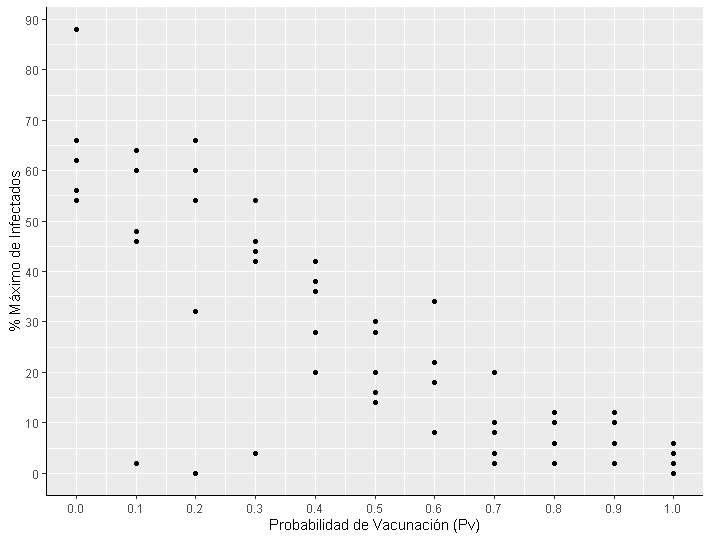
\includegraphics[width=0.6\linewidth]{Rplot1}
	\caption{\% Máximo de infectados alcanzado}
	\label{fig:imagen1}
\end{figure}

Por otro lado, estableciendo la relación que se tiene del porcentaje de vacunación con el que son creados los agentes y el momento (iteración) en la que se alcanza el máximo porcentaje de contagios, se puede comentar que, aunque no es claro el comportamiento general se puede identificar lo siguiente: 
\begin{enumerate}
\item Para valores intermedios de $Pv (0.3 < Pv <0.8)$ el porcentaje máximo de contagios se alcanza en momentos tardíos de la corrida. 
\item En valores altos de porcentaje de vacunación $(0.7 < Pv)$ el porcentaje máximo de contagios se alcanza en momentos tempranos de la corrida, esto se puede deber a que se tienen muchos menos contagios.
\end{enumerate}



\begin{figure}[h]
	\centering
	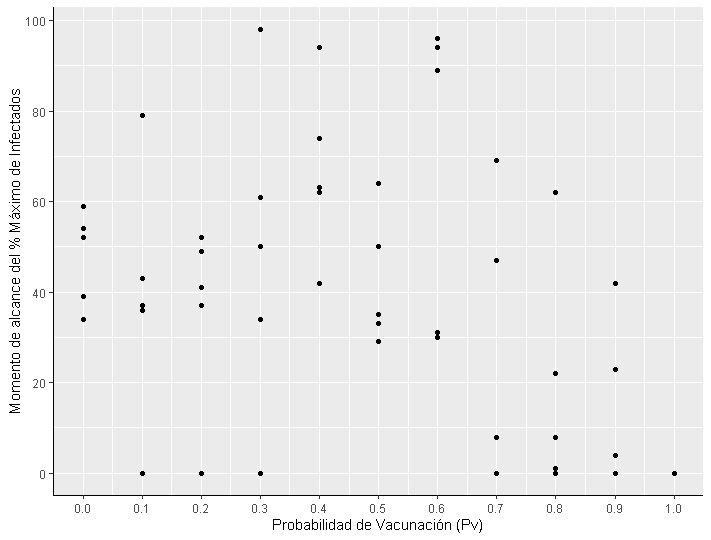
\includegraphics[width=0.6\linewidth]{Rplot2}
	\caption{Momento (iteración) en la que se alcanza el \% máximo de infectados}
	\label{fig:imagen2}
\end{figure}

Finalmente, y como extra, se presenta una gráfica en la que se relaciona el porcentaje de vacunación utilizado en la creación de un agente contra el total de iteraciones que se tuvieron que realizar porque aún había agentes contagiados.  Cabe mencionar que, si el número de iteraciones fue $100$, significa que se alcanzó el criterio de paro de $100$ iteraciones pero que aún había agentes infectados. Se puede inferir que en valores altos de porcentaje de vacunación $(0.7 < Pv)$ el porcentaje máximo de contagios se alcanza en momentos tempranos de la corrida, además de que no se necesitan las $100$ iteraciones ya que en momento más temprano se queda el experimento sin agentes que puedan seguir propagando la infección.

\begin{figure}[h]
	\centering
	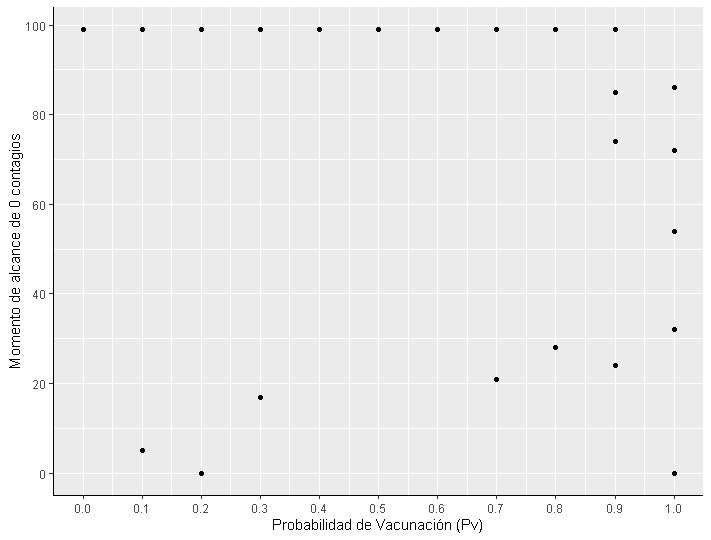
\includegraphics[width=0.6\linewidth]{Rplot3}
	\caption{Iteraciones con mas de 0 infectados}
	\label{fig:imagen3}
\end{figure}
\newpage
\section{Conclusión}
Tomando como referencia los resultados mostrados en las gráficas podemos presentar las siguientes conclusiones con respecto al modelo SIR con la variante de vacunación en el momento de creación de los agentes:
\begin{enumerate}

\item A mayor probabilidad de vacunación en la creación de cada agente, menor es el porcentaje máximo de contagiados alcanzado.
\item Para valores intermedios de $Pv (0.3 < Pv <0.8)$ el porcentaje máximo de contagios (pico de la infección) se alcanza en momentos tardíos de la corrida. 
\item En valores altos de porcentaje de vacunación $(0.7 < Pv)$ el porcentaje máximo de contagios se alcanza en momentos tempranos de la corrida, esto se puede deber a que se tienen muchos menos contagios.
\item En valores altos de porcentaje de vacunación $(0.7 < Pv)$ el porcentaje máximo de contagios se alcanza en momentos tempranos de la corrida, además de que no se necesitan las 100 iteraciones ya que en momento más temprano se queda el experimento sin agentes que puedan seguir propagando la infección.

\end{enumerate}
\bibliography{Biblio}
\bibliographystyle{plainnat}


\end{document}
	
	
	
	